\chapter{Methodology}
\section{Thin Film Fabrication}
Thirty glass substrates, measuring $1"\times0.25"$, were cut from microscope slides.
These substrates were subject to three successive ionic layer adhesion and reaction (SILAR) processes (Table \ref{tab:processes}).
All of the SILAR processes consist of a certain number of deposition cycles from a fixed precursor solution with $0.095M$ Zn$^{2+}$ and $0.190M$ NaOH and a thermal annealing at certain temperatures \cite{gao08, florido17}.

\begin{table}
  \caption[SILAR Processes]{Processing parameters manipulated and SILAR processes}
  \centering
  \begin{tabular}{c c c c}
    \hline\hline
     & S1 & S2 & S3 \\
    \hline
    Depostion cycles & 100 & 75 & 100 \\
    Annealing temperature & 450$\degg$C & 450$\degg$C & 500$\degg$C \\[1ex]
    \hline
  \end{tabular}
  \label{tab:processes}
\end{table}

\section{Thin Film Characterization}
The fabricated thin films were characterized for determination of thin film structure and properties.
One thin film fabricated using each of the fabrication processes was chosen for optical microscopy.
The fabricated material was split into four sections as shown in Figure \ref{fig:orient}.
The sections were chosen such that the four corners of the rectangular substrate represent different probe volumes.
The thin films were viewed under the high power objective lens ($400\times$) of a digital compound microscope.

\begin{figure}
  \centering
  \begin{tabular}{| c | c |}
    \hline
    1 & 3 \\
    \hline
    2 & 4 \\[0.5ex]
    \hline
  \end{tabular}
  \caption{Basic orientation matrix}
  \label{fig:orient}
\end{figure}

Overall thin film structure were also characterized with x-ray diffraction, using Cu-K$\alpha$ anode ($\lambda = \SI{1.54}{\angstrom}$), and scanning electron microscopy at varying magnifications for crystal growth verification, lateral view assessment, and distribution analysis.
<<<<<<< HEAD
=======

>>>>>>> Edit metho accrdg to sirs comments
Finally, the thin films sheet resistance values were derived from measurements from four-point probe sensing.
The schematic for the four-point probe mechanism are shown in Figure \ref{fig:fpt}.

\begin{figure}
  \centering
  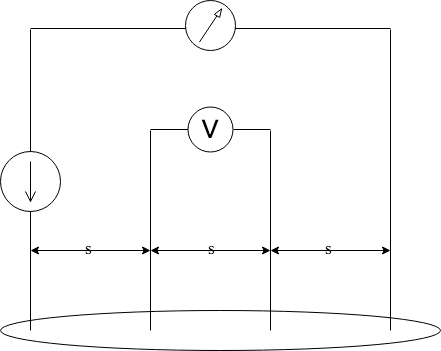
\includegraphics[scale=0.3]{FourPoint}
  \caption{Four point probe mechanism for determination of sheet resistance}
  \label{fig:fpt}
\end{figure}

\section{Model creation and data analysis}
There are a total of two discrete microstructure functions (DMF) that are studied.
The dimensions of the probe volume $V$ were chosen as odd products of small primes (2, 3, 5, and 7) to aid in the computation of two point spatial correlations.
Two point spatial correlations were derived from optical microscopy imges through the definition of measures \cite{gupta15}.

\[
  m^{np}_r = \dfrac{1}{S_rN} \sum_{i=0}^{N} \sum_{i=0}^{R} m^p_r m^n_r
\]

where $n$ and $p$ are the discrete local states of interest and $r$ is the spatial bin of interest.

Image data were transformed into Julia 2D arrays \cite{julia15} and further into a user defined data structure named \emph{MaterialImage} which accounts for the parameters used for defining the DMFs.
There are a total of 20 sets two point spatial correlations that will be considered.

Since the preferred orientation of the fabrication of thin films is unknown, each of the three thin films have four hypothesized orientations based on circular permuations of the orientation matrix (Figure \ref{fig:orient}).

For each of the calculated two point spatial correlations, the values have undergone principal component analysis to obtain the orthogonal latent descriptors \cite{gupta15, sun17}.
This is done with \emph{MultivariateStats.jl}, a package available for multivariate statistical analysis \cite{mvstats}.
Optimal orientation is determined when the variance of the dimensionally-reduced two point statistics, \textit{i.e. the matrix trace of the covariance matrix} is minimized.

\subsection{Determination of optimal microstructure function}
The plots for the two-point statistics were manually compared.
Partial least squares analysis (PLSA) was done to compare the ability of the DMF to capture the variation of derived sheet resistance values.
Evaluation of the optimal microstructure function was based on the following parameters: variance capture using PLSA and qualitative assessment of clustering of microstructure ensembles.
